\begin{figure}[!htbp]
	\centering
	\resizebox{0.9\textwidth}{!}{%
		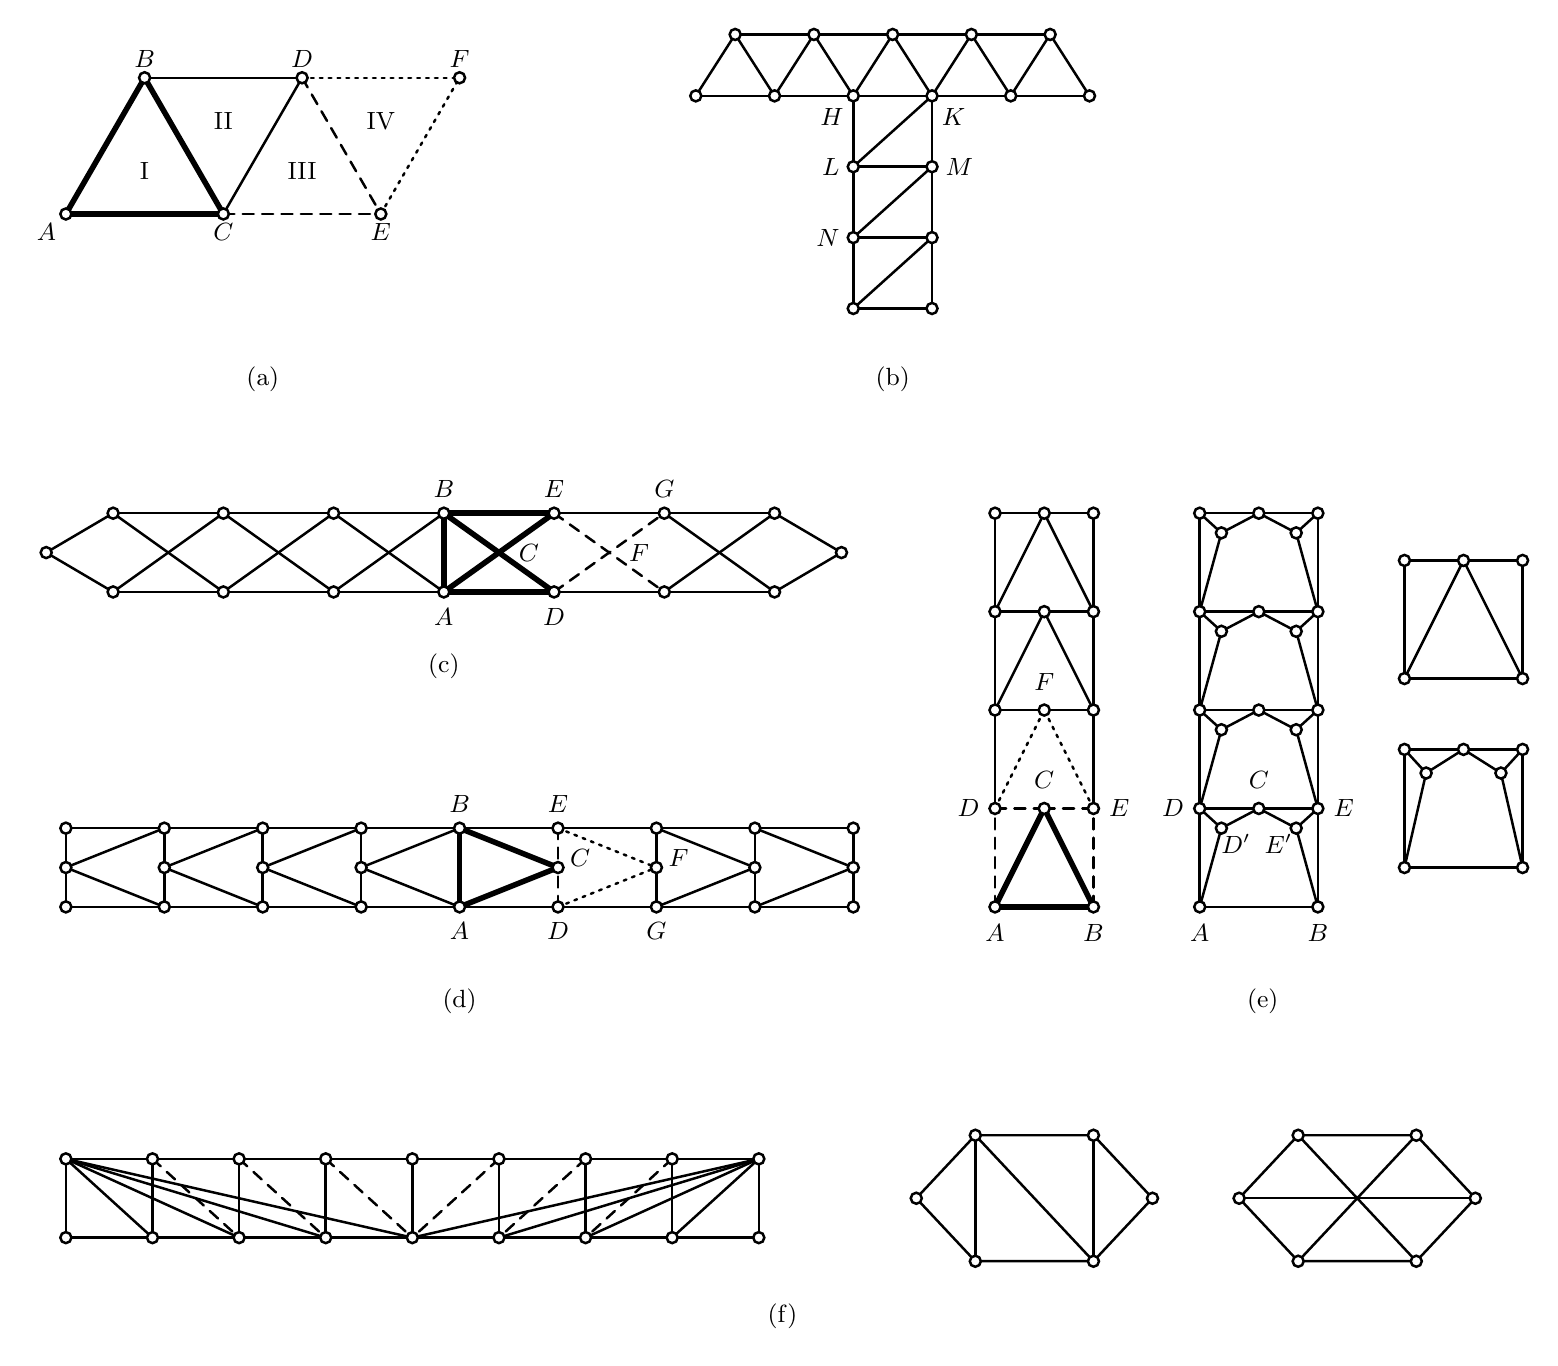
\begin{tikzpicture}[
			asta/.style={line width=0.9pt, line cap=round, line join=round, black},
			base/.style={line width=2.0pt, line cap=round, line join=round, black},
			nuova/.style={line width=0.9pt, line cap=round, line join=round, black,
				dash pattern=on 4pt off 3pt},
			futura/.style={line width=0.9pt, line cap=round, black,
				dash pattern=on 1pt off 2.2pt},
			nodo/.style={circle, fill=white, draw=black,
				inner sep=0pt, minimum size=4.0pt, line width=0.9pt},
			etich/.style={font=\small},
			pan/.style={font=\small},
			]
			
			%% =========================================================
			%% (a) COMPOSIZIONE GERARCHICA A MAGLIE TRIANGOLARI
			%% =========================================================
			\begin{scope}[xshift=0cm, yshift=-1.0cm]
				\coordinate (aA) at (0,0);
				\coordinate (aC) at (2,0);
				\coordinate (aB) at (1,1.73);
				\coordinate (aD) at (3,1.73);
				\coordinate (aE) at (4,0);
				\coordinate (aF) at (5,1.73);
				%% maglia I (base)
				\draw[base](aA)--(aC)--(aB)--cycle;
				%% maglia II
				\draw[asta](aB)--(aD);
				\draw[asta](aC)--(aD);
				%% maglia III
				\draw[nuova](aC)--(aE);
				\draw[nuova](aD)--(aE);
				%% maglia IV
				\draw[futura](aD)--(aF);
				\draw[futura](aE)--(aF);
				\foreach \n in {aA,aB,aC,aD,aE,aF} \node[nodo]at(\n){};
				\node[etich,below left ]at(aA){$A$};
				\node[etich,above      ]at(aB){$B$};
				\node[etich,below      ]at(aC){$C$};
				\node[etich,above      ]at(aD){$D$};
				\node[etich,below      ]at(aE){$E$};
				\node[etich,above      ]at(aF){$F$};
				\node[etich]at(1.00,0.55){I};
				\node[etich]at(2.00,1.18){II};
				\node[etich]at(3.00,0.55){III};
				\node[etich]at(4.00,1.18){IV};
				\node[pan]at(2.5,-2.10){(a)};
			\end{scope}
			
			%% =========================================================
			%% (b) TRAVATURA RAMIFICATA
			%% =========================================================
			\begin{scope}[xshift=8.0cm, yshift=0.5cm]
				%% travatura orizzontale (Warren)
				\draw[asta](0,0)--(5,0);
				\draw[asta](0.5,0.78)--(4.5,0.78);
				\foreach \i in {0,...,4}{
					\draw[asta](\i,0)--(\i+0.5,0.78);
					\draw[asta](\i+0.5,0.78)--(\i+1,0);}
				%% ramo verticale dall'asta HK
				\draw[asta](2,0)--(2,-2.7);
				\draw[asta](3,0)--(3,-2.7);
				\draw[asta](2,-0.9)--(3,-0.9);
				\draw[asta](2,-1.8)--(3,-1.8);
				\draw[asta](2,-2.7)--(3,-2.7);
				\draw[asta](2,-0.9)--(3,0);
				\draw[asta](2,-1.8)--(3,-0.9);
				\draw[asta](2,-2.7)--(3,-1.8);
				%% nodi
				\foreach \i in {0,...,5} \node[nodo]at(\i,0){};
				\foreach \i in {0,...,4} \node[nodo]at(\i+0.5,0.78){};
				\foreach \y in {-0.9,-1.8,-2.7}{
					\node[nodo]at(2,\y){}; \node[nodo]at(3,\y){};}
				%% etichette
				\node[etich,below left ]at(2,-0.04){$H$};
				\node[etich,below right]at(3,-0.04){$K$};
				\node[etich,left ]at(1.95,-0.9){$L$};
				\node[etich,right]at(3.05,-0.9){$M$};
				\node[etich,left ]at(1.95,-1.8){$N$};
				\node[pan]at(2.5,-3.60){(b)};
			\end{scope}
			
			%% =========================================================
			%% (c) MAGLIE ROMBOIDALI
			%% =========================================================
			\begin{scope}[xshift=0.6cm, yshift=-5.8cm]
				\def\dc{1.4}
				%% correnti
				\draw[asta](0,0)--(6*\dc,0);
				\draw[asta](0,1)--(6*\dc,1);
				%% estremita' a punta
				\draw[asta](-0.85,0.5)--(0,1);
				\draw[asta](-0.85,0.5)--(0,0);
				\draw[asta](6*\dc+0.85,0.5)--(6*\dc,1);
				\draw[asta](6*\dc+0.85,0.5)--(6*\dc,0);
				%% diagonali incrociate (campate non in evidenza)
				\foreach \i in {0,1,2,5}{
					\draw[asta](\i*\dc,0)--(\i*\dc+\dc,1);
					\draw[asta](\i*\dc,1)--(\i*\dc+\dc,0);}
				%% maglia generatrice in evidenza: montante AB + campata ABED
				\draw[base](3*\dc,0)--(3*\dc,1);
				\draw[base](3*\dc,0)--(4*\dc,0);
				\draw[base](3*\dc,1)--(4*\dc,1);
				\draw[base](3*\dc,0)--(4*\dc,1);
				\draw[base](3*\dc,1)--(4*\dc,0);
				%% passo successivo: diagonali D-G ed E-H (tratteggiate)
				\draw[nuova](4*\dc,0)--(5*\dc,1);
				\draw[nuova](4*\dc,1)--(5*\dc,0);
				%% passo ancora successivo: correnti E-G e D-H (punteggiati)
				\draw[futura](4*\dc,1)--(5*\dc,1);
				\draw[futura](4*\dc,0)--(5*\dc,0);
				%% nodi
				\foreach \i in {0,...,6}{
					\node[nodo]at(\i*\dc,0){}; \node[nodo]at(\i*\dc,1){};}
				\node[nodo]at(-0.85,0.5){};
				\node[nodo]at(6*\dc+0.85,0.5){};
				%% etichette (C ed F: incroci senza nodo strutturale)
				\node[etich,below]at(3*\dc,-0.08){$A$};
				\node[etich,above]at(3*\dc, 1.08){$B$};
				\node[etich]at(3.5*\dc+0.38,0.50){$C$};
				\node[etich,below]at(4*\dc,-0.08){$D$};
				\node[etich,above]at(4*\dc, 1.08){$E$};
				\node[etich]at(4.5*\dc+0.38,0.50){$F$};
				\node[etich,above]at(5*\dc, 1.08){$G$};
				\node[pan]at(3*\dc,-0.95){(c)};
			\end{scope}
			
			%% =========================================================
			%% (d.1) MAGLIE A K --- travatura orizzontale
			%% =========================================================
			\begin{scope}[xshift=0cm, yshift=-9.8cm]
				\def\dk{1.25}
				%% correnti
				\draw[asta](0,0)--(8*\dk,0);
				\draw[asta](0,1)--(8*\dk,1);
				%% montanti
				\foreach \i in {0,1,2,3,4,6,7,8}
				\draw[asta](\i*\dk,0)--(\i*\dk,1);
				%% diagonali a K: meta' sinistra convergenti a sinistra
				\foreach \i in {0,1,2,3}{
					\draw[asta]({(\i+1)*\dk},0)--(\i*\dk,0.5);
					\draw[asta]({(\i+1)*\dk},1)--(\i*\dk,0.5);}
				%% meta' destra: campate gia' composte
				\foreach \i in {6,7}{
					\draw[asta](\i*\dk,0)--({(\i+1)*\dk},0.5);
					\draw[asta](\i*\dk,1)--({(\i+1)*\dk},0.5);}
				%% generazione in evidenza: triangolo A-B-C
				\draw[base](4*\dk,0)--(4*\dk,1);
				\draw[base](4*\dk,0)--(5*\dk,0.5);
				\draw[base](4*\dk,1)--(5*\dk,0.5);
				%% passo successivo: nodi D, E (correnti + mezzi montanti)
				\draw[nuova](4*\dk,0)--(5*\dk,0);
				\draw[nuova](4*\dk,1)--(5*\dk,1);
				\draw[nuova](5*\dk,0)--(5*\dk,0.5);
				\draw[nuova](5*\dk,1)--(5*\dk,0.5);
				%% passo ancora successivo: nodi F, G
				\draw[futura](5*\dk,0)--(6*\dk,0.5);
				\draw[futura](5*\dk,1)--(6*\dk,0.5);
				\draw[futura](5*\dk,0)--(6*\dk,0);
				\draw[futura](6*\dk,0)--(6*\dk,0.5);
				%% nodi
				\foreach \i in {0,...,8}{
					\node[nodo]at(\i*\dk,0){}; \node[nodo]at(\i*\dk,1){};}
				\foreach \i in {0,1,2,3,5,6,7,8} \node[nodo]at(\i*\dk,0.5){};
				%% etichette
				\node[etich,below]at(4*\dk,-0.08){$A$};
				\node[etich,above]at(4*\dk, 1.08){$B$};
				\node[etich]at(5*\dk+0.28,0.62){$C$};
				\node[etich,below]at(5*\dk,-0.08){$D$};
				\node[etich,above]at(5*\dk, 1.08){$E$};
				\node[etich]at(6*\dk+0.28,0.62){$F$};
				\node[etich,below]at(6*\dk,-0.08){$G$};
			\end{scope}
			
			%% =========================================================
			%% (e.1) TORRI A K --- variante con nodo sul traverso
			%% =========================================================
			\begin{scope}[xshift=11.8cm, yshift=-9.8cm, scale=1.25]
				%% concio generativo
				\draw[base](0,0)--(1,0);
				\draw[base](0,0)--(0.5,1);
				\draw[base](1,0)--(0.5,1);
				\draw[nuova](0,0)--(0,1);
				\draw[nuova](1,0)--(1,1);
				\draw[nuova](0,1)--(0.5,1);
				\draw[nuova](1,1)--(0.5,1);
				\draw[futura](0,1)--(0.5,2);
				\draw[futura](1,1)--(0.5,2);
				%% conci superiori
				\draw[asta](0,1)--(0,4);
				\draw[asta](1,1)--(1,4);
				\draw[asta](0,2)--(1,2);
				\draw[asta](0,3)--(1,3);
				\draw[asta](0,4)--(1,4);
				\draw[asta](0,2)--(0.5,3);
				\draw[asta](1,2)--(0.5,3);
				\draw[asta](0,3)--(0.5,4);
				\draw[asta](1,3)--(0.5,4);
				%% nodi
				\foreach \y in {0,...,4}{
					\node[nodo]at(0,\y){}; \node[nodo]at(1,\y){};}
				\foreach \y in {1,...,4} \node[nodo]at(0.5,\y){};
				%% etichette
				\node[etich,below]at(0,-0.08){$A$};
				\node[etich,below]at(1,-0.08){$B$};
				\node[etich,left ]at(-0.06,1){$D$};
				\node[etich,right]at(1.06,1){$E$};
				\node[etich,above]at(0.5,1.10){$C$};
				\node[etich,above]at(0.5,2.10){$F$};
			\end{scope}
			
			%% =========================================================
			%% (e.2) TORRI A K --- variante a diagonali simmetriche
			%% =========================================================
			\begin{scope}[xshift=14.4cm, yshift=-9.8cm, scale=1.25]
				\foreach \k in {0,...,3}{
					\begin{scope}[yshift=\k cm]
						\draw[asta](0,0)--(0,1);
						\draw[asta](1.2,0)--(1.2,1);
						\draw[asta](0,1)--(0.6,1);
						\draw[asta](0.6,1)--(1.2,1);
						\draw[asta](0,0)--(0.22,0.80);
						\draw[asta](0.22,0.80)--(0,1);
						\draw[asta](0.22,0.80)--(0.6,1);
						\draw[asta](1.2,0)--(0.98,0.80);
						\draw[asta](0.98,0.80)--(1.2,1);
						\draw[asta](0.98,0.80)--(0.6,1);
				\end{scope}}
				\draw[asta](0,0)--(1.2,0);
				%% nodi
				\foreach \y in {0,...,4}{
					\node[nodo]at(0,\y){}; \node[nodo]at(1.2,\y){};}
				\foreach \y in {1,...,4} \node[nodo]at(0.6,\y){};
				\foreach \k in {0,...,3}{
					\node[nodo]at(0.22,{\k+0.80}){};
					\node[nodo]at(0.98,{\k+0.80}){};}
				%% etichette
				\node[etich,below]at(0,-0.08){$A$};
				\node[etich,below]at(1.2,-0.08){$B$};
				\node[etich,left ]at(-0.06,1){$D$};
				\node[etich,right]at(1.26,1){$E$};
				\node[etich,above]at(0.6,1.10){$C$};
				\node[etich,right]at(0.12,0.64){$D'$};
				\node[etich,below]at(0.80,0.84){$E'$};
			\end{scope}
			
			%% =========================================================
			%% (e.3) maglie elementari delle due varianti
			%% =========================================================
			\begin{scope}[xshift=17.0cm, yshift=-6.9cm, scale=1.25]
				%% maglia con nodo sul traverso
				\draw[asta](0,0)--(1.2,0)--(1.2,1.2)--(0,1.2)--cycle;
				\draw[asta](0,0)--(0.6,1.2);
				\draw[asta](1.2,0)--(0.6,1.2);
				\foreach \p in {(0,0),(1.2,0),(0,1.2),(0.6,1.2),(1.2,1.2)}
				\node[nodo]at\p{};
			\end{scope}
			\begin{scope}[xshift=17.0cm, yshift=-9.3cm, scale=1.25]
				%% maglia a diagonali simmetriche
				\draw[asta](0,0)--(1.2,0)--(1.2,1.2)--(0,1.2)--cycle;
				\draw[asta](0,0)--(0.22,0.96);
				\draw[asta](0.22,0.96)--(0,1.2);
				\draw[asta](0.22,0.96)--(0.6,1.2);
				\draw[asta](1.2,0)--(0.98,0.96);
				\draw[asta](0.98,0.96)--(1.2,1.2);
				\draw[asta](0.98,0.96)--(0.6,1.2);
				\foreach \p in {(0,0),(1.2,0),(0,1.2),(0.6,1.2),(1.2,1.2),
					(0.22,0.96),(0.98,0.96)}
				\node[nodo]at\p{};
			\end{scope}
			
			\node[pan]at(5.0,-11.0){(d)};
			
			\node[pan]at(15.2,-11.0){(e)};
			
			%% =========================================================
			%% (f.1) SCHEMA IBRIDO: diagonali a ventaglio
			%% =========================================================
			\begin{scope}[xshift=0cm, yshift=-14.0cm]
				\def\de{1.1}
				\draw[asta](0,0)--(8*\de,0);
				\draw[asta](0,1)--(8*\de,1);
				\foreach \i in {0,...,8} \draw[asta](\i*\de,0)--(\i*\de,1);
				%% ventaglio dalle estremita' superiori
				\foreach \j in {1,2,3,4} \draw[asta](0,1)--(\j*\de,0);
				\foreach \j in {7,6,5,4} \draw[asta](8*\de,1)--(\j*\de,0);
				%% aste sostituite (tratteggiate)
				\foreach \i in {1,2,3} \draw[nuova](\i*\de,1)--({(\i+1)*\de},0);
				\foreach \i in {7,6,5} \draw[nuova](\i*\de,1)--({(\i-1)*\de},0);
				\foreach \i in {0,...,8}{
					\node[nodo]at(\i*\de,0){}; \node[nodo]at(\i*\de,1){};}
			\end{scope}
			
			%% =========================================================
			%% (f.2) SCHEMI IBRIDI ESAGONALI
			%% =========================================================
			\begin{scope}[xshift=10.8cm, yshift=-14.3cm]
				\coordinate (hL)  at (0,0.8);
				\coordinate (htl) at (0.75,1.6);
				\coordinate (htr) at (2.25,1.6);
				\coordinate (hR)  at (3,0.8);
				\coordinate (hbr) at (2.25,0);
				\coordinate (hbl) at (0.75,0);
				\draw[asta](hL)--(htl)--(htr)--(hR)--(hbr)--(hbl)--cycle;
				\draw[asta](htl)--(hbl);
				\draw[asta](htl)--(hbr);
				\draw[asta](htr)--(hbr);
				\foreach \n in {hL,htl,htr,hR,hbr,hbl} \node[nodo]at(\n){};
			\end{scope}
			\begin{scope}[xshift=14.9cm, yshift=-14.3cm]
				\coordinate (kL)  at (0,0.8);
				\coordinate (ktl) at (0.75,1.6);
				\coordinate (ktr) at (2.25,1.6);
				\coordinate (kR)  at (3,0.8);
				\coordinate (kbr) at (2.25,0);
				\coordinate (kbl) at (0.75,0);
				\draw[asta](kL)--(ktl)--(ktr)--(kR)--(kbr)--(kbl)--cycle;
				\draw[asta](kL)--(kR);
				\draw[asta](ktl)--(kbr);
				\draw[asta](ktr)--(kbl);
				\foreach \n in {kL,ktl,ktr,kR,kbr,kbl} \node[nodo]at(\n){};
			\end{scope}
			
			\node[pan]at(9.1,-15.0){(f)};
			
	\end{tikzpicture}}
	\caption{Tipologie di maglie nelle travature reticolari
		piane isostatiche.
		(a): composizione gerarchica a maglie
		triangolari; i nodi sono aggiunti progressivamente
		e le aste nuove sono tratteggiate.
		(b): travatura ramificata, ottenuta
		avviando la composizione da un'asta intermedia
		anziché da un nodo.
		(c): maglie romboidali; le diagonali
		si incrociano senza nodo strutturale.
		(d): maglie a K, con i montanti spezzati
		a metà altezza dal nodo su cui convergono
		le diagonali.
		(e): varianti a torre della maglia a K,
		con nodo sul traverso e a diagonali simmetriche;
		a fianco le rispettive maglie elementari.
		(f): schemi ibridi con aste di parete
		non standard: nello schema a ventaglio le aste
		tratteggiate sono le diagonali dello schema
		triangolare di partenza, soppresse e sostituite
		dalle aste uscenti a ventaglio dai nodi estremi
		del corrente superiore.}
	\label{fig:tipologie_maglie}
\end{figure}
